\section{Tutorial B11}

\begin{problem}
    Find the natural domain of the function $f$ for the following:
    \begin{enumerate}
        \item $f(x, y) = \sqrt{1 - x^2 - y^2}$
        \item $f(x, y) = \ln{x^2 - y}$
        \item $f(x, y) = \arcsin{x + y}$
        \item $f(x, y) = \frac1{x^2 - y^2}$
    \end{enumerate}
\end{problem}
\begin{solution}
    \begin{ppart}
        Observe that the argument of the square root must be non-negative. Hence, $1 - x^2 - y^2 \geq 0 \implies x^2 + y^2 \leq 1$. Thus, \[\dom f = \{ (x, y) \in \RR^2 : x^2 + y^2 \leq 1\}.\]
    \end{ppart}
    \begin{ppart}
        Observe that the argument of the natural log must be positive. Hence, $x^2 - y > 0 \implies y < x^2$. Thus, \[\dom f = \{(x, y) \in \RR^2 : y < x^2\}.\]
    \end{ppart}
    \begin{ppart}
        Observe that the argument of $\arcsin$ must be within the range of $\sin$, i.e. between $-1$ and 1 inclusive. Hence, $-1 \leq x + y \leq 1$. Thus, \[\dom f = \{(x, y) \in \RR^2 : -1 \leq x + y \leq 1\}.\]
    \end{ppart}
    \begin{ppart}
        Observe that the denominator must be non-zero. Hence, $x^2 - y^2 \neq 0 \implies y^2 \neq x^2 \implies y \neq x \lor y \neq -x$. Thus, \[\dom f = \{(x, y) \in \RR^2 : y \neq x \lor y \neq -x\}.\]
    \end{ppart}
\end{solution}

\begin{problem}
    Identify the correct equations of the following surfaces in 3-D space.

    \begin{itemize}
        \item $z = \cos{x + y}$
        \item $z = x^2y + 1$
        \item $z = 3 - x + y$
        \item $z = -\frac1{\sqrt{x^2 + y^2}}$
    \end{itemize}

    \begin{enumerate}
        \item \begin{center}\tikzsetnextfilename{207}
            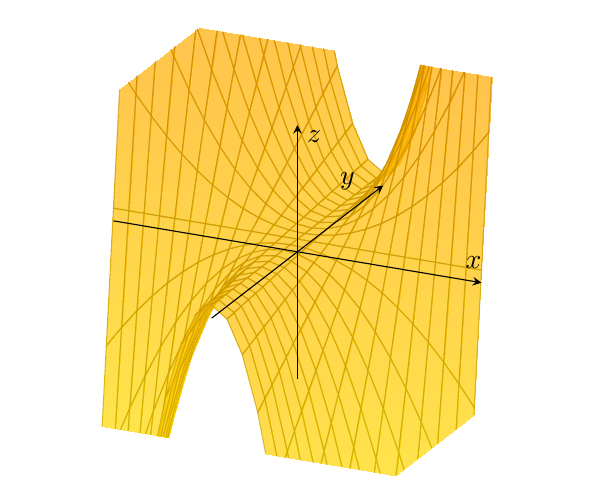
\begin{tikzpicture}[trim axis left, trim axis right]
                \begin{axis}[
                    axis on top,
                    axis y line=middle,
                    axis x line=middle,
                    axis z line=middle,
                    xtick = \empty,
                    ytick = \empty,
                    ztick = \empty,
                    xlabel = {$x$},
                    ylabel = {$y$},
                    zlabel = {$z$},
                    zmax = 10,
                    zmin = -10,
                    legend cell align={left},
                    legend pos=outer north east,
                    ]
                    \addplot3[surf,shader=faceted interp, colormap/hot,opacity=0.7]{x^2 * y + 1};
                \end{axis}
            \end{tikzpicture}
        \end{center}
        \item \begin{center}\tikzsetnextfilename{208}
            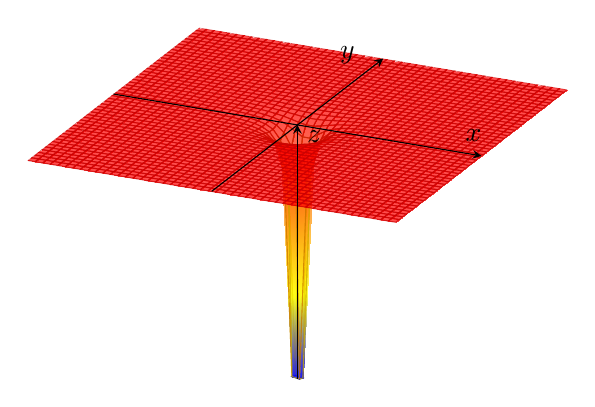
\begin{tikzpicture}[trim axis left, trim axis right]
                \begin{axis}[
                    axis on top,
                    axis y line=middle,
                    axis x line=middle,
                    axis z line=middle,
                    xtick = \empty,
                    ytick = \empty,
                    ztick = \empty,
                    xlabel = {$x$},
                    ylabel = {$y$},
                    zlabel = {$z$},
                    samples=50,
                    legend cell align={left},
                    legend pos=outer north east,
                    ]
                    \addplot3[surf,shader=faceted interp, colormap/hot,opacity=0.7, ]{-1/(x^2 + y^2)};
                \end{axis}
            \end{tikzpicture}
        \end{center}
        \item \begin{center}\tikzsetnextfilename{209}
            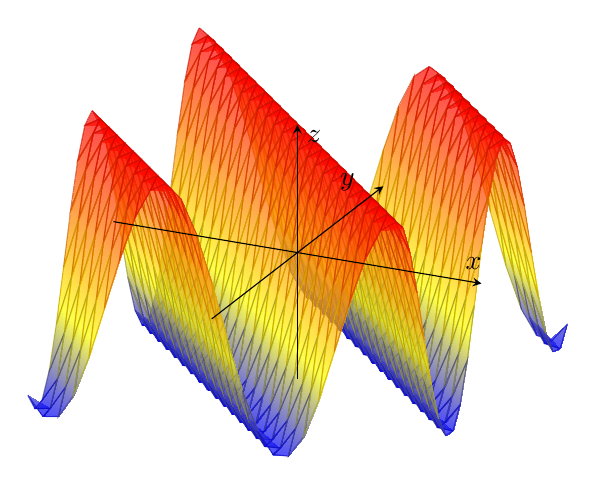
\begin{tikzpicture}[trim axis left, trim axis right]
                \begin{axis}[
                    axis on top,
                    axis y line=middle,
                    axis x line=middle,
                    axis z line=middle,
                    xtick = \empty,
                    ytick = \empty,
                    ztick = \empty,
                    xlabel = {$x$},
                    ylabel = {$y$},
                    zlabel = {$z$},
                    legend cell align={left},
                    legend pos=outer north east,
                    ]
                    \addplot3[surf,shader=faceted interp, colormap/hot,opacity=0.7, ]{cos(\x r + \y r)};
                \end{axis}
            \end{tikzpicture}
        \end{center}
        \item \begin{center}\tikzsetnextfilename{210}
            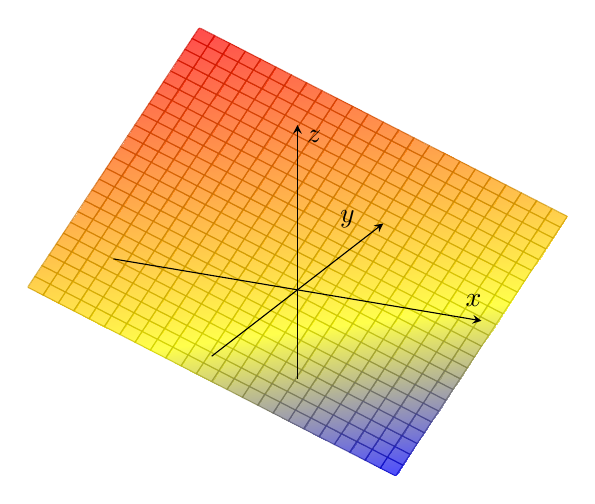
\begin{tikzpicture}[trim axis left, trim axis right]
                \begin{axis}[
                    axis on top,
                    axis y line=middle,
                    axis x line=middle,
                    axis z line=middle,
                    xtick = \empty,
                    ytick = \empty,
                    ztick = \empty,
                    xlabel = {$x$},
                    ylabel = {$y$},
                    zlabel = {$z$},
                    legend cell align={left},
                    legend pos=outer north east,
                    ]
                    \addplot3[surf,shader=faceted interp, colormap/hot,opacity=0.7, ]{3 - x + y};
                \end{axis}
            \end{tikzpicture}
        \end{center}
    \end{enumerate}
\end{problem}
\begin{solution}
    \begin{ppart}
        $z = x^2 y + 1$
    \end{ppart}
    \begin{ppart}
        $z = -\frac1{\sqrt{x^2 + y^2}}$
    \end{ppart}
    \begin{ppart}
        $z = \cos{x + y}$
    \end{ppart}
    \begin{ppart}
        $z = 3 - x + y$
    \end{ppart}
\end{solution}

\begin{problem}
    Let $f(x, y) = x^2 - 2x^3 + 3xy$. Find an equation of the level curve that passes through the point
    \begin{enumerate}
        \item $(-1, 1)$
        \item $(2, -1)$
        \item $(1, 5)$
    \end{enumerate}
\end{problem}
\begin{solution}
    \begin{ppart}
        Note that $f(-1, 1) = 0$. Hence, the level curve is given by \[x^2 - 2x^3 + 3xy = 0.\]
    \end{ppart}
    \begin{ppart}
        Note that $f(2, -1) = -18$. Hence, the level curve is given by \[x^2 - 2x^3 + 3xy = -18.\]
    \end{ppart}
    \begin{ppart}
        Note that $f(1, 5) = 14$. Hence, the level curve is given by \[x^2 - 2x^3 + 3xy = 14.\]
    \end{ppart}
\end{solution}

\begin{problem}
    If $V(x, y)$ is the voltage or potential at a point $(x, y)$ in the $xy$-plane, then the level curves of $V$ are called equipotential curves. Along such a curve, the voltage remains constant. Given that \[V(x, y) = \frac{8}{\sqrt{16 + x^2 + y^2}}\] find an equation of the equipotential curves at which
    \begin{enumerate}
        \item $V = 2.0$
        \item $V = 1.0$
        \item $V = 0.5$
    \end{enumerate}
\end{problem}
\begin{solution}
    Rearranging the given equation, we have \[x^2 + y^2 = \frac{64}{V^2} - 16.\]

    \begin{ppart}
        When $V = 2.0$, we have $x^2 + y^2 = \frac{64}{2.0^2} - 16 = 0$, whence \[x = 0 \land y = 0.\]
    \end{ppart}
    \begin{ppart}
        When $V = 1.0$, we have \[x^2 + y^2 = \frac{64}{1.0^2} - 16 = 48.\]
    \end{ppart}
    \begin{ppart}
        When $V = 0.5$, we have \[x^2 + y^2 = \frac{64}{0.5^2} - 16 = 240.\]
    \end{ppart}
\end{solution}

\begin{problem}
    Given that $f(x, y) = x^4 \sin{xy^3}$, find $f_x(x, y)$, $f_y(x, y)$, $f_{xy}(x, y)$ and $f_{yx}(x, y)$.
\end{problem}
\begin{solution}
    Differentiating $f$ with respect to $x$, \[f_x(x, y) = 4x^3 \sin{xy^3} + x^4 y^3 \cos{xy^3}.\]

    Differentiating $f$ with respect to $y$, \[f_y(x, y) = 3x^5y^2\cos{xy^3}.\]

    Differentiating $f_x$ with respect to $y$, 
    \begin{align*}
        f_{xy}(x, y) &= 12x^4y^2\cos{xy^3} + x^4\bs{3y^2\cos{xy^3} - 3xy^5\sin{xy^3}}\\
        &= 15x^4y^2\cos{xy^3} - 3x^5y^5\sin{xy^3}.
    \end{align*}

    Differentiating $f_y$ with respect to $x$,
    \begin{align*}
        f_{yx}(x, y) &= 3y^2\bs{5x^4 \cos{xy^3} - x^5y^3\sin{xy^3}}\\
        &= 15x^4y^2 \cos{xy^3} - 3x^5y^5 \sin{xy^3}.
    \end{align*}
\end{solution}

\begin{problem}
    Given that $z = x^2y$, $x = t^2$, $y = t^3$, use the chain rule to find $\der{z}{t}$ in terms of $t$.
\end{problem}
\begin{solution}
    \[\der{z}{t} = \pder{z}{x} \cdot \der{x}{t} + \pder{z}{y} \cdot \der{y}{t} = 2xy \bp{2t} + x^2 \bp{3t^2} = 2t^2t^3 \cdot 2t + \bp{t^2}^2 \cdot 3t^2 = 7t^6.\]
\end{solution}

\begin{problem}
    Find the gradient of $f(x, y) = 3x^2y$ at the point $(1, 2)$ and use it to calculate the directional derivative of $f$ at $(1, 2)$ in the direction of the vector $\vec u = 3\vec i + 4\vec j$.
\end{problem}
\begin{solution}
    Note that $f_x(x, y) = 6xy$ and $f_y(x, y) = 3x^2$. Hence, $\nabla f$ at $(1, 2)$ is $\cveciix{12}{3}$. 
            
    Observe that the directional derivative of $f$ in the direction of $\vec u$ at $(1, 2)$ is given by \[\nabla f \cdot \hat{\vec u} = \cvecii{12}3 \cdot \frac15 \cvecii34 = \frac{48}5.\] Thus, the instantaneous rate of change at $(1, 2)$ in the direction of $\vec u$ is $48/5$.
\end{solution}

\begin{problem}
    Suppose that a point moves along the intersection of the sphere $x^2 + y^2 + z^2 = 1$ with the plane $x = \frac23$. Find the rate of $z$ with respect to $y$ when the point is at $\bp{\frac23, \frac13, \frac23}$.
\end{problem}
\begin{solution}
    Note that $x^2 + y^2 + z^2 = 1 \implies z = \pm \sqrt{1 - x^2 - y^2}$. Given that the object we want (the rate of change of $z$ with respect to $y$) will later be evaluated when $z = \frac23 > 0$, we consider only the positive branch. Let $f(x, y) = \sqrt{1 - x^2 - y^2}$. Then $f_y(x, y) = \frac{-y}{\sqrt{1 - x^2 - y^2}}$. Evaluating at the desired point, we get, \[f_y\bp{\frac23, \frac13} = \frac{-1/3}{\sqrt{1 - (2/3)^2 - (1/3)^2}} = -\frac12.\]
\end{solution}

\begin{problem}
    \begin{enumerate}
        \item The Cauchy-Riemann equations are such that $\pderx{u}{x} = \pderx{v}{y}$ and $\pderx{u}{y} = -\pderx{v}{x}$ for $u(x, y)$ and $v(x, y)$. Show that $u = \e^x \cos y$, $v = \e^x \sin y$ satisfy the Cauchy-Riemann equations.
        \item Show that the function $f(x, y) = \e^x \sin y + \e^y \cos x$ satisfies that Laplace equation, i.e. $\pderx[2]{f}{x} + \pderx[2]{f}{y} = 0$.
        \item If $u(x, y)$ and $v(x, y)$ satisfy the Cauchy-Riemann equations, state the conditions for both $u$ and $v$ to satisfy the Laplace equation.
    \end{enumerate}
\end{problem}
\begin{solution}
    \begin{ppart}
        Differentiating $u$ with respect to $x$, we get $\pderx{u}{x} = \e^x \cos y$. Differentiating $v$ with respect to $y$, we get $\pderx{v}{y} = \e^x \cos y$. Hence, $\pderx{u}{x} = \pderx{v}{y}$.

        Differentiating $u$ with respect to $y$, we get $\pderx{u}{y} = -\e^x \sin y$. Differentiating $v$ with respect to $x$, we get $\pderx{v}{x} = \e^x \sin y$. Hence, $\pderx{u}{y} = -\pderx{v}{x}$.
        
        Thus, $u$ and $v$ satisfy the Cauchy-Riemann equations.
    \end{ppart}
    \begin{ppart}
        Differentiating $f$ twice with respect to $x$, \[\pder[2]{f}{x} = \pder{}{x} (\e^x \sin y - \e^y \sin x) = \e^x \sin y - \e^y \cos x.\] Differentiating $f$ twice with respect to $y$, \[\pder[2]{f}{y} = \pder{}{y} (\e^x \cos y + \e^y \cos x) = -\e^x \sin y + \e^y \cos x.\] Hence,\[\pder[2]{f}{x} + \pder[2]{f}{y} = \bp{\e^x \sin y - \e^y \cos x} + \bp{-\e^x \sin y + \e^y \cos x} = 0.\] Thus, $f(x, y) = \e^x \sin y + \e^y \cos x$ satisfies the Laplace equation.
    \end{ppart}
    \begin{ppart}
        Suppose $u(x, y)$ and $v(x, y)$ satisfy the Cauchy-Riemann equations. This gives
        \[\begin{cases}
            \begin{aligned}
                u_x &= v_y\\
                u_y &= -v_x
            \end{aligned}
        \end{cases}
        \]
        Differentiating with respect to $x$ and $y$, we obtain
        \[\begin{cases}
            \begin{aligned}
                u_{xx} &= v_{yx}\\
                u_{yx} &= -v_{xx}
            \end{aligned}
        \end{cases} \quad \land \qquad \begin{cases}
            \begin{aligned}
                u_{xy} &= v_{yy}\\
                u_{yy} &= -v_{xy}
            \end{aligned}
        \end{cases}\] This gives
        \[\begin{cases}
            \begin{aligned}
                u_{xx} + u_{yy} &= v_{yx} - v_{xy}\\
                v_{xx} + v_{yy} &= -u_{yx} + u_{xy}\\
            \end{aligned}
        \end{cases}
        \]
        Hence, if $u$ and $v$ both satisfy the Laplace equation, we require 
        \[\begin{cases}
            \begin{aligned}
                v_{yx} - v_{xy} &= 0\\
                -u_{yx} + u_{xy} &= 0\\
            \end{aligned}
        \end{cases}
        \]
        which gives the conditions $u_{xy} = u_{yx}$ and $v_{xy} = v_{yx}$.
    \end{ppart}
\end{solution}

\begin{problem}
    Find the equation of the tangent plane to the surface $z = x^2 y$ at the point $(2, 1, 4)$. Hence, state the normal vector of the tangent plane.
\end{problem}
\begin{solution}
    Let $f(x, y) = x^2y$. Then $f_x(x, y) = 2xy$ and $f_y(x, y) = x^2$. Hence, the equation of the tangent plane at $(2, 1, 4)$ is given by \[z = 4 + f_x(2, 1)(x-2) + f_y(2, 1)(y - 1) = 4 + 4(x-2) + 4(y-1) = 4x + 4y - 8.\] Rearranging, \[4x + 4y - z = 8,\] whence the normal vector of the tangent plane is $\cveciiix44{-1}$.
\end{solution}

\begin{problem}
    The volume of a right-circular cone of radius $r$ cm and height $h$ cm is denoted by $V$. If $h$ increases from $10$ cm to $10.01$ cm and $r$ decreases from $12$ cm to $11.95$ cm, use a linear approximation to estimate the volume of the cone after the changes.
\end{problem}
\begin{solution}
    Let $V(r, h) = \frac13 \pi r^2 h$ be the volume of the cone. We have $V_r(r, h) = \frac23 \pi r h$ and $V_h(r, h) = \frac13 \pi r^2$. The equation of the tangent plane at $r = 12$ and $h = 10$ is given by
    \begin{gather*}
        v = V(12, 10) + V_r(12, 10)(r-12) + V_h(12, 10)(h-10)\\
        = \frac13\pi(12^2)(10) + \frac23 \pi(12)(10)(r - 12) + \frac13 \pi (12^2) (h-10) = 16\pi(5r + 3h - 60).
    \end{gather*}
    Evaluating at $r = 11.95$ and $h = 10.01$, we have
    \[v = 16\pi\bs{5(11.95) + 3(10.01) - 60} = 476.48\pi.\] The volume of the cone after the changes is hence approximately $476.48\pi$ cm$^3$.
\end{solution}

\begin{problem}
    The radius of a right-circular cylinder is measured with an error of at most $2\%$, and the height is measured with an error of at most 4\%. Approximate the maximum possible percentage error in the volume of the cylinder calculated from these measurements.
\end{problem}
\begin{solution}
    Let the volume of the cylinder be $V = \pi r^2 h$. By the chain rule, we have \[\d V = \pder{V}{r} \d r + \pder{f}{h} \d h = 2\pi rh \d  r + \pi r^2 \d h.\] Dividing throughout by $V = \pi r^2 h$, \[\frac{\d V}{V} = \frac{2\pi rh \d  r + \pi r^2 \d h}{\pi r^2 h} = 2 \frac{\d r}{r} + \frac{\d h}{h}.\] Note that $\d V / V$ measures the percentage error of the volume $V$, while $\d r / r$ and $\d h / h$ measure the percentage error of the radius and height respectively. Hence, \[\max \frac{\d V}{V} = 2(2\%) + 4\% = 8\%.\]
\end{solution}

\begin{problem}
    On a certain mountain, the elevation $z$ above a point $(x, y)$ in a horizontal $xy$-plane that lies at sea level is $z = 2000 - 2x^2 - 4y^2$ ft. The positive $x$-axis points east, and the positive $y$-axis points north. A climber is at the point $(-20, 5, 1100)$.

    \begin{enumerate}
        \item If the climber uses a compass reading to walk due northeast, will he ascend or descend? Find this rate.
        \item Find the direction where the climber should walk to travel a level path.
    \end{enumerate}
\end{problem}
\begin{solution}
    \begin{ppart}
        Let $f(x, y) = 2000 - 2x^2 - 4y^2$. Then $f_x(x, y) = -4x$ and $f_y(x, y) = -8y$. Hence, \[\nabla f = \cvecii{-4x}{-8y} = -4\cvecii{x}{2y}\] Note that the vector $\cveciix11$ points northeast. \[\nabla f \cdot \widehat{\cvecii11} = -4\cvecii{x}{2y} \cdot \frac{\sqrt2}{2} \cvecii11 = -2\sqrt2 \bp{x + 2y}.\] Evaluating at $(-20, 5, 1100)$, the instantaneous rate of change of the climber's altitude would be $-2\sqrt2\bp{-20 + 2\cdot5} = 20\sqrt2$ ft/s. That is, the climber would ascend at a rate of $20\sqrt2$ feet per second.
    \end{ppart}
    \begin{ppart}
        For a level path, the instantaneous rate of change of the climber's altitude should be 0. Let the direction of the climber be $u = \cveciix{a}{b}$. \[\evalder{D_{\vec u} f(x, y)}{(-20, 5)} = -4\cvecii{-20}{10} \cdot \cvecii{a}{b} \implies -2a + b = 0 \implies b = 2a.\] We hence have \[\vec u = \cvecii{a}{b} = \cvecii{a}{2a} = a\cvecii12.\] Thus, the climber should walk in the direction of $\cveciix{1}{2}$.
    \end{ppart}
\end{solution}

\begin{problem}
    Find the absolute maximum and minimum values of $f(x, y) = 3xy - 6x - 3y + 7$ on the closed triangular region $R$ with vertices $(0, 0)$, $(3, 0)$ and $(0, 5)$.
\end{problem}
\begin{solution}
    Note that $f_x(x, y) = 3y - 6$ and $f_y(x, y) = 3x - 3$, whence $f_{xx}(x, y) = f_{yy}(x, y) = 0$ and $f_{xy} = 3$. For stationary points, \[\nabla f = \vec 0 \implies \cvecii{3y-6}{3x-3} = \vec 0 \implies x = 1, \, y = 2.\]

    Consider the nature of the stationary point at $(1, 2)$. We have \[D = f_{xx}(1, 2)f_{yy}(1, 2) - \bs{f_{xy}(1, 2)}^2 = -9 < 0\] Hence, by the second derivative test, we see that $f(x, y)$ has a saddle point at $(1, 2)$. Thus, the extrema of $f(x, y)$ must occur along its boundary.

    Note that the boundary of $f(x, y)$ is given by
    \begin{itemize}
        \item $x = 0$, $y \in [0, 5]$
        \item $x \in [0, 3]$, $y = 0$
        \item $x \in [0, 3]$, $y = 5 - \frac53 x$
    \end{itemize}

    \case{1}[$x = 0$, $y \in [0,5]$] We have that $f(0, y) = -3y + 7$, which clearly attains a maximum of 7 at $y = 0$ and a minimum of $-8$ at $y = 5$.

    \case{2}[$x \in [0, 3]$, $y = 0$] We have that $f(x, 0) = -6x + 7$, which clearly attains a maximum of 7 at $x = 0$ and a minimum of $-11$ at $x = 3$.

    \case{3}[$x \in [0, 3]$, $y = 5 - \frac53 x$] Observe that \[f\of{x, 5 - \frac53 x} = 3x\bp{5 - \frac53 x} - 6x - 3\bp{5 - \frac53 x} + 7 = -(x-2)(5x-4)\] is concave down and has a turning point at $x = 1.4$. Hence, the function clearly attains a maximum of $1.8$ when $x = 1.4$ and a minimum of $-11$ when $x = 3$ (note that at $x = 0$, the function returns $-8$). 

    Hence, the maximum of $f(x, y)$ is 7, while the minimum is $-11$.
\end{solution}

\begin{problem}
    Find the dimensions of a rectangular box, open at the top, having a volume of 32 cm$^3$, and requiring the least amount of material for its construction.
\end{problem}
\begin{solution}
    Let the box have side lengths of $x$, $y$ and $z$ cm. Given that the volume of the box is fixed at 32 cm$^3$, we have \[xyz = 32 \implies z = \frac{32}{xy}\] Let the surface area of the box be measured by $f(x, y)$. Then \[f(x, y) = xy + 2yz + 2xz = xy + 2y\bp{\frac{32}{xy}} + 2x\bp{\frac{32}{xy}} = xy + 64x^{-1} + 64y^{-1}.\] Note that \[\nabla f = \cvecii{f_x(x, y)}{f_y(x, y)} = \cvecii{y-64x^{-2}}{x - 64y^{-2}}.\] For stationary points, $\nabla f = \vec 0$. We hence obtain
    \[
        \begin{cases}
            y = 64x^{-2}\\
            x = 64y^{-2}
        \end{cases} \implies
        \begin{cases}
            yx^2 = 64\\
            xy^2 = 64
        \end{cases}
        \implies x^3y^3 = 64^2 \implies xy = 16
    \]
    Hence, \[x = \frac{x^2y}{xy} = \frac{64}{16} = 4,\] whence $y = 4$ and $z = 2$. Thus, $f(x, y)$ has a stationary point at $(4, 4, 2)$. 
    
    We now consider the nature of this stationary point. Note that \[f_{xx}(x, y) = 128x^{-3}, \quad f_{yy} = 128y^{-3},\quad f_{xy} = 1.\] Hence, \[D = f_{xx}(4, 4)f_{yy}(4, 4) - \bs{f_{xy}(4, 4)}^2 = 3\] Since $D > 0$ and $f_{xx}(4, 4) = 2 > 0$, by the second derivative test, $f(x, y)$ attains a minimum at $(4, 4, 2)$. Thus, the amount of material required is lowest for a box of dimension $4 \times 4 \times 2$.
\end{solution}

\clearpage
\begin{problem}
    Find the quadratic approximation of $f(x, y) = x^2 y + xy^2$ around the point $(1, 1)$.
\end{problem}
\begin{solution}
    Taking partial derivatives, we have
    \begin{gather*}
        f_x(x, y) = 2xy + y^2, \quad f_y(x, y) = 2xy + x^2\\
        f_{xx}(x, y) = 2y, \quad f_{xy}(x, y) = 2x + 2y, \quad f_{yy}(x, y) = 2x.
    \end{gather*}
    Hence, the required quadratic approximation $Q(x, y)$ is given by
    \begin{align*}
        Q(x, y) &= f(1, 1) + f_x(1, 1)(x-1) + f_y(1, 1)(y-1)\\
        & \hspace{3em} + \frac12 f_{xx}(1, 1)(x-1)^2 + f_{xy}(1, 1)(x-1)(y-1) + \frac12 f_{yy}(1, 1)(y-1)^2\\
        &= 2 + 3(x - 1) + 3(y - 1) + (x-1)^2 + 4(x-1)(y-1) + (y-1)^2\\
        &= 2 - 3x - 3y + 4xy + x^2 + y^2
    \end{align*}
\end{solution}